\documentclass[12pt,letterpaper]{article}

\usepackage[margin=0.85in]{geometry}
\usepackage[T1]{fontenc}
\usepackage{lmodern}
\usepackage[scaled=0.95]{helvet}
\renewcommand{\familydefault}{\sfdefault}
\usepackage{amsmath}
\usepackage{array}
\usepackage{tabularx}
\usepackage[table]{xcolor}
\usepackage{tikz}
\usetikzlibrary{arrows.meta}
\usepackage[most]{tcolorbox}
\usepackage{titlesec}
\usepackage{fancyhdr}
\usepackage{needspace}
\usepackage{enumitem}

% ---------- Colors ----------
\definecolor{monster}{HTML}{1F6FB5}   % Cookie Monster blue
\definecolor{cookiedark}{HTML}{7A4A22}
\definecolor{elmo}{HTML}{D32F2F}
\definecolor{abby}{HTML}{C2185B}      % Abby Cadabby pink, darkened for print
\definecolor{oscar}{HTML}{4C8C2B}
\definecolor{count}{HTML}{6B3FA0}     % The Count purple
\definecolor{cookie}{HTML}{C68B4E}
\definecolor{chip}{HTML}{3B2314}
\definecolor{softyellow}{HTML}{FFF6DD}
\definecolor{softblue}{HTML}{E8F1FA}
\definecolor{softpurple}{HTML}{F1EBF8}
\definecolor{softgreen}{HTML}{EDF5E8}
\definecolor{gold}{HTML}{C68B4E}

% ---------- Headings ----------
\titleformat{\section}{\Large\bfseries\color{cookiedark}}{}{0pt}{}
\titlespacing*{\section}{0pt}{14pt}{6pt}
\setcounter{secnumdepth}{0}

\pagestyle{fancy}
\fancyhf{}
\renewcommand{\headrulewidth}{0pt}
\fancyfoot[C]{\small\color{gray}Elmo's Cookie Waves \textperiodcentered\ page \thepage}

\setlength{\parindent}{0pt}
\setlength{\parskip}{6pt}

% ---------- Helpers ----------
% A cookie with chocolate chips
\newcommand{\cookie}[1][1]{%
  \begin{tikzpicture}[scale=#1, baseline=-0.6ex]
    \fill[cookie] (0,0) circle (0.5);
    \draw[cookiedark, line width=0.8pt] (0,0) circle (0.5);
    \foreach \x/\y in {-0.2/0.2, 0.15/0.25, 0.25/-0.1, -0.1/-0.25, -0.28/-0.05, 0.05/0.0}
      \fill[chip] (\x,\y) circle (0.06);
  \end{tikzpicture}}

% Empty wave grid: x = 0..8 eighths of a lap, y = -4..4 squares
\newcommand{\wavegrid}{%
  \draw[step=1, gray!30] (0,-4) grid (8,4);
  \draw[-{Stealth}, line width=0.8pt] (0,0) -- (8.6,0) node[right, font=\small, align=left] {time\\(eighths\\of a lap)};
  \draw[-{Stealth}, line width=0.8pt] (0,-4.2) -- (0,4.6) node[above, font=\small] {height};
  \foreach \x in {0,...,8} \node[below, font=\scriptsize] at (\x,-4) {\x};
  \foreach \y in {-4,...,4} \node[left, font=\scriptsize] at (0,\y) {\y};}

\newcommand{\blank}[1][3cm]{\underline{\hspace{#1}}}

\newcounter{question}
\newcommand{\question}{%
  \refstepcounter{question}\par\needspace{3\baselineskip}%
  \textbf{\color{monster}Question \arabic{question}.}~}

\newtcolorbox{bigidea}[1][]{enhanced, colback=softyellow, colframe=gold,
  boxrule=1pt, arc=3mm, left=8pt, right=8pt, top=6pt, bottom=6pt, #1}
\newtcolorbox{tryit}{enhanced, colback=softblue, colframe=monster,
  boxrule=0.8pt, arc=3mm, left=8pt, right=8pt}
\newtcolorbox{mathclub}[1]{enhanced, colback=softpurple, colframe=count,
  boxrule=0.8pt, arc=3mm, left=8pt, right=8pt, top=4pt, bottom=4pt,
  title={\textbf{#1}}, colbacktitle=count, coltitle=white}
\newtcolorbox{radiobox}[1]{enhanced, colback=softgreen, colframe=oscar,
  boxrule=0.8pt, arc=3mm, left=8pt, right=8pt, top=4pt, bottom=4pt,
  title={\textbf{#1}}, colbacktitle=oscar, coltitle=white}

\renewcommand{\arraystretch}{1.6}

\begin{document}

% ================= Title =================
\begin{center}
  {\cookie[0.9]\hspace{0.6em}\cookie[0.9]\hspace{0.6em}\cookie[0.9]}\\[6pt]
  {\Huge\bfseries\color{cookiedark} Elmo's Cookie Waves}\\[4pt]
  {\Large Euler's Equation Makes Waves, and What Phase Means}\\[6pt]
  {\small\color{gray} November 4, 2026 \textperiodcentered\ Nathaniel}
\end{center}

\vspace{2pt}
Name: \blank[6cm] \hfill Date: \blank[4cm]

% ================= The story =================
\section{The story}

In The Cookie Circle, \textbf{\color{elmo}Elmo} walked around the edge of Cookie Monster's
giant cookie. Now Elmo keeps walking, around and around, at the same speed.
\textbf{\color{count}The Count} shines a flashlight from the side, so Elmo's
\textbf{shadow} moves up and down on the wall.

\emph{``Elmo is going around and around. But Elmo's shadow goes up and down!''}

That up-and-down shadow is a \textbf{wave}. Radios, phones, Wi-Fi, light, and sound are all
made of waves like this. Let's draw one.

% ================= Elmo's shadow =================
\section{Elmo's shadow on the wall}

The cookie is drawn on a grid. Its edge is \textbf{4 squares} from the middle. Elmo starts at
spot \textbf{0} and walks around to the left (up first), stopping at each numbered spot. Each
spot is \textbf{one eighth} of a lap. The dashed lines show his shadow's height on the wall.

\begin{center}
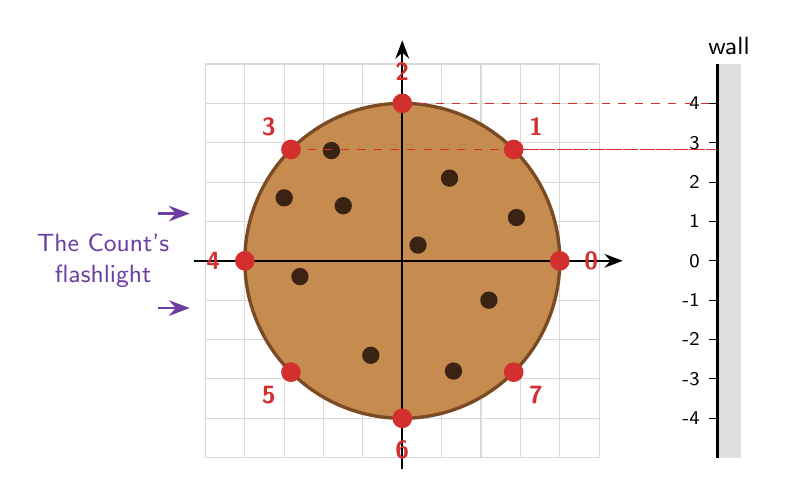
\begin{tikzpicture}[scale=0.5]
  \draw[step=1, gray!30] (-5,-5) grid (5,5);
  \fill[cookie] (0,0) circle (4);
  \foreach \x/\y in {-1.5/1.4, 1.2/2.1, 2.2/-1, -0.8/-2.4, -2.6/-0.4, 0.4/0.4, 1.3/-2.8, -1.8/2.8, 2.9/1.1, -3/1.6}
    \fill[chip] (\x,\y) circle (0.22);
  \draw[cookiedark, line width=1.2pt] (0,0) circle (4);
  \draw[-{Stealth}, line width=0.8pt] (-5.3,0) -- (5.6,0);
  \draw[-{Stealth}, line width=0.8pt] (0,-5.3) -- (0,5.6);
  % wall
  \fill[gray!25] (8,-5) rectangle (8.6,5);
  \draw[line width=1pt] (8,-5) -- (8,5);
  \node[above, font=\small] at (8.3,5) {wall};
  \foreach \y in {-4,...,4} {
    \draw (7.8,\y) -- (8,\y);
    \node[left, font=\scriptsize] at (7.8,\y) {\y};
  }
  % spots
  \foreach \k in {0,...,7} {
    \pgfmathsetmacro{\a}{45*\k}
    \fill[elmo] ({4*cos(\a)},{4*sin(\a)}) circle (0.25);
    \node[font=\small\bfseries, elmo] at ({4.8*cos(\a)},{4.8*sin(\a)}) {\k};
  }
  \foreach \k in {1,2,3} {
    \pgfmathsetmacro{\a}{45*\k}
    \draw[dashed, elmo] ({4*cos(\a)},{4*sin(\a)}) -- (8,{4*sin(\a)});
  }
  % flashlight
  \node[font=\small, align=center, count] at (-7.6,0) {The Count's\\flashlight};
  \draw[-{Stealth}, count, line width=1pt] (-6.2,1.2) -- (-5.4,1.2);
  \draw[-{Stealth}, count, line width=1pt] (-6.2,-1.2) -- (-5.4,-1.2);
\end{tikzpicture}
\end{center}

\question Fill in Elmo's shadow height at each spot. Use the grid and the wall. (Spots 1, 3, 5
and 7 are a little less than 3 squares, so write ``about 3.'')

\begin{center}
\renewcommand{\arraystretch}{1.5}
\begin{tabular}{|l|*{9}{>{\centering\arraybackslash}p{0.95cm}|}}
\hline
\rowcolor{elmo}
\textbf{\color{white}Spot} & \textbf{\color{white}0} & \textbf{\color{white}1} & \textbf{\color{white}2} & \textbf{\color{white}3} & \textbf{\color{white}4} & \textbf{\color{white}5} & \textbf{\color{white}6} & \textbf{\color{white}7} & \textbf{\color{white}8} \\ \hline
\textbf{Height} & 0 & 3 & 4 & & & & & & \\ \hline
\end{tabular}
\end{center}

{\small Spot 8 is back at the start: one whole lap!}

% ================= Draw the wave =================
\newpage
\section{Draw the wave}

\question Put a \textbf{\color{elmo}red} dot for each height from your table: spot number across,
height up. Then connect the dots with a smooth, curvy line.

\begin{center}
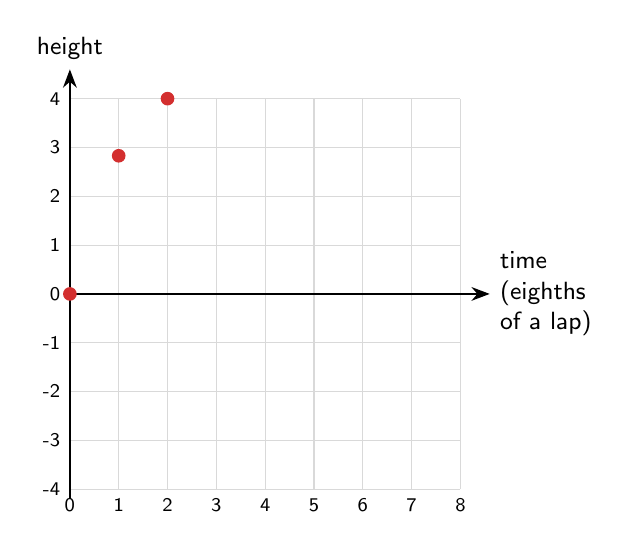
\begin{tikzpicture}[scale=0.62]
  \wavegrid
  \fill[elmo] (0,0) circle (0.14);
  \fill[elmo] (1,2.83) circle (0.14);
  \fill[elmo] (2,4) circle (0.14);
\end{tikzpicture}
\end{center}

\begin{bigidea}
Going \textbf{around} a circle makes a \textbf{wave} that goes \textbf{up and down}! This wave
has a name: the \textbf{sine wave} (say ``sign''). Every lap around the cookie draws one more
bump up and one more dip down.
\end{bigidea}

\section{Three words engineers use}

\begin{center}
\renewcommand{\arraystretch}{1.7}
\begin{tabularx}{\linewidth}{|>{\bfseries}p{2.7cm}|X|}
\hline
\rowcolor{cookiedark}
\textbf{\color{white}Word} & \textbf{\color{white}What it means for Elmo} \\ \hline
Amplitude & How \textbf{tall} the wave is. It is the size of the cookie: how far the edge is
from the middle. \\ \hline
Frequency & How many \textbf{laps} Elmo walks every second. The Count counts them:
\emph{``ONE lap! TWO laps! THREE laps in one second! Ah ah ah!''} That is 3 \textbf{hertz}. \\ \hline
Phase & \textbf{Where on the circle} you are, or how far \textbf{ahead} one walker is of another.
We measure it in turns, or in degrees: a whole turn is $360^\circ$. \\ \hline
\end{tabularx}
\end{center}

\question The wave's highest point is \blank[1.5cm] squares. So its amplitude is
\blank[1.5cm].

\vspace{4pt}
\question A radio station at 100 megahertz makes its wave go around \textbf{100 million} laps
every second! If Elmo walks 5 laps in one second, his frequency is \blank[1.5cm] hertz.

% ================= Phase =================
\newpage
\section{Phase: Abby starts ahead}

\textbf{\color{abby}Abby Cadabby} wants to walk too. But Abby starts at spot \textbf{2}, at the
\textbf{top} of the cookie, a \textbf{quarter turn ahead} of Elmo. They walk at the same speed.

\question Fill in Abby's height when Elmo is at each spot. (Abby is always 2 spots ahead.)

\begin{center}
\renewcommand{\arraystretch}{1.5}
\begin{tabular}{|l|*{9}{>{\centering\arraybackslash}p{0.95cm}|}}
\hline
\rowcolor{abby}
\textbf{\color{white}Elmo's spot} & \textbf{\color{white}0} & \textbf{\color{white}1} & \textbf{\color{white}2} & \textbf{\color{white}3} & \textbf{\color{white}4} & \textbf{\color{white}5} & \textbf{\color{white}6} & \textbf{\color{white}7} & \textbf{\color{white}8} \\ \hline
\textbf{Abby's height} & 4 & 3 & & & & & & & \\ \hline
\end{tabular}
\end{center}

\question Draw Abby's wave in \textbf{\color{abby}pink} on the grid. Elmo's wave is already
there.

\begin{center}
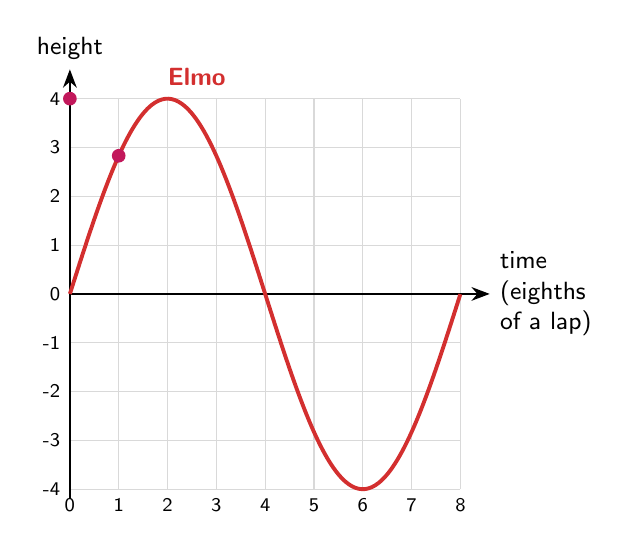
\begin{tikzpicture}[scale=0.62]
  \wavegrid
  \draw[elmo, line width=1.4pt, domain=0:8, samples=120, smooth] plot (\x, {4*sin(45*\x)});
  \node[elmo, font=\small\bfseries] at (2.6,4.45) {Elmo};
  \fill[abby] (0,4) circle (0.14);
  \fill[abby] (1,2.83) circle (0.14);
\end{tikzpicture}
\end{center}

\question Abby's wave looks just like Elmo's, but \textbf{slid over}. Whose wave reaches the
top first? \blank[2.5cm]

\begin{bigidea}
Abby's wave is the same wave, \textbf{shifted}. That shift is called the \textbf{phase}. Abby is
a quarter turn ahead, so her phase is $\boldsymbol{90^\circ}$ ahead of Elmo's. Engineers say the
two waves are \textbf{$\boldsymbol{90^\circ}$ out of phase}.
\end{bigidea}

\question Fill in the phase for each turn.

\begin{center}
\renewcommand{\arraystretch}{1.6}
\begin{tabular}{|>{\centering\arraybackslash}p{3.4cm}|>{\centering\arraybackslash}p{3.4cm}|}
\hline
\rowcolor{count}
\textbf{\color{white}How far ahead} & \textbf{\color{white}Phase} \\ \hline
quarter turn & $90^\circ$ \\ \hline
half turn & \\ \hline
three-quarters turn & \\ \hline
whole turn & \\ \hline
\end{tabular}
\end{center}

% ================= Oscar cancels =================
\newpage
\section{Oscar's opposite wave}

\textbf{\color{oscar}Oscar the Grouch} starts at spot \textbf{4}, a \textbf{half turn}
($180^\circ$) ahead. When Elmo's shadow goes up, Oscar's goes down. \emph{``Scram!''}

\question Fill in Oscar's heights, then \textbf{add} Elmo's and Oscar's heights together.

\begin{center}
\renewcommand{\arraystretch}{1.5}
\begin{tabular}{|l|*{9}{>{\centering\arraybackslash}p{0.95cm}|}}
\hline
\rowcolor{cookiedark}
\textbf{\color{white}Spot} & \textbf{\color{white}0} & \textbf{\color{white}1} & \textbf{\color{white}2} & \textbf{\color{white}3} & \textbf{\color{white}4} & \textbf{\color{white}5} & \textbf{\color{white}6} & \textbf{\color{white}7} & \textbf{\color{white}8} \\ \hline
\textbf{\color{elmo}Elmo} & 0 & 3 & 4 & 3 & 0 & $-3$ & $-4$ & $-3$ & 0 \\ \hline
\textbf{\color{oscar}Oscar} & 0 & $-3$ & & & & & & & \\ \hline
\textbf{Elmo $+$ Oscar} & 0 & 0 & & & & & & & \\ \hline
\end{tabular}
\end{center}

\question What happens when you add two waves that are a half turn apart?\\[4pt]
\blank[8cm]

\begin{bigidea}
Waves a half turn apart \textbf{cancel}: together they make \textbf{nothing}! Waves that start
together (\textbf{in phase}) \textbf{add up} to a bigger wave. This is called
\textbf{interference}.
\end{bigidea}

\question Elmo's twin walks right next to him, in phase. Add their heights at spot 2:
$4 + 4 = $ \blank[1.5cm]. The new wave is \blank[2cm] (taller or shorter?).

\begin{radiobox}{How engineers use phase}
\begin{itemize}[leftmargin=1.2em, itemsep=2pt, topsep=2pt]
\item \textbf{Noise-canceling headphones} listen to the noise and play the same wave a half turn
  ahead, so the noise cancels.
\item \textbf{Antennas} working together add their waves in phase in one direction, so the radio
  hears farther, and cancel in other directions.
\item \textbf{Radios} send messages by changing the phase of a wave: a little turn ahead or
  behind means a different message.
\end{itemize}
\end{radiobox}

% ================= Euler =================
\section{Back to Euler's equation}

\begin{mathclub}{The Count's Math Club: Euler's wave equation}
In The Cookie Circle, $e^{\,j\,\times\,\text{steps}}$ meant ``walk that many steps around the
circle.'' Engineers write the steps as $\theta$ (the Greek letter ``theta''). Euler showed:
\[
  e^{j\theta} = \underbrace{\cos\theta}_{\text{floor shadow}} \;+\; j\,\underbrace{\sin\theta}_{\text{wall shadow}}
\]
The \textbf{wall shadow} is the sine wave you drew. The \textbf{floor shadow} (a flashlight from
above) is the \textbf{cosine wave}, which is Abby's wave! Radio engineers call these two shadows
\textbf{I} and \textbf{Q}.
\end{mathclub}

\begin{bigidea}
\textbf{The big secret: a phase shift is a turn you multiply by.} Abby is a quarter turn ahead
of Elmo. A quarter turn is $j$! So
\[
  \text{Abby} = j \times \text{Elmo}.
\]
Oscar is a half turn ahead: $\text{Oscar} = -1 \times \text{Elmo}$. That is why his wave is
upside down, and why Elmo $+$ Oscar $= 0$.
\end{bigidea}

\question Which number do you multiply by to shift a wave a quarter turn? \blank[1.5cm]
\quad A half turn? \blank[1.5cm]

\begin{center}
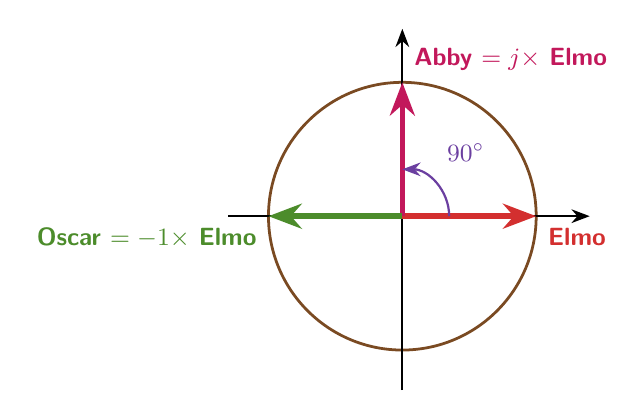
\begin{tikzpicture}[scale=0.85]
  \draw[cookiedark, line width=1pt] (0,0) circle (2);
  \draw[-{Stealth}, line width=0.8pt] (-2.6,0) -- (2.8,0);
  \draw[-{Stealth}, line width=0.8pt] (0,-2.6) -- (0,2.8);
  \draw[-{Stealth}, elmo, line width=2pt] (0,0) -- (2,0) node[below right, font=\small\bfseries] {Elmo};
  \draw[-{Stealth}, abby, line width=2pt] (0,0) -- (0,2) node[above right, font=\small\bfseries] {Abby $= j \times$ Elmo};
  \draw[-{Stealth}, oscar, line width=2pt] (0,0) -- (-2,0) node[below left, font=\small\bfseries] {Oscar $= -1 \times$ Elmo};
  \draw[-{Stealth}, count, line width=0.8pt] (0.7,0) arc (0:90:0.7);
  \node[count, font=\small] at (0.95,0.95) {$90^\circ$};
\end{tikzpicture}
\end{center}

\begin{bigidea}
Engineers draw each wave as an \textbf{arrow} on the cookie, called a \textbf{phasor}. The arrow's
\textbf{length} is the amplitude. The arrow's \textbf{direction} is the phase. As time goes by,
all the arrows spin around together, like Elmo, Abby, and Oscar walking. One arrow tells you
everything about a wave!
\end{bigidea}

\begin{tcolorbox}[enhanced, colback=white, colframe=monster, boxrule=1pt, arc=3mm,
  height=4.3cm, title={\textbf{Draw it!}}, colbacktitle=monster, coltitle=white]
Draw a cookie with three arrows for Elmo, Abby, and Oscar. Next to it, draw their three waves.
\end{tcolorbox}

{\small\color{gray}\textbf{For teachers:} Elmo's position after angle $\theta = \omega t$ is
$4e^{j\omega t}$; his wall shadow is $4\sin\omega t$ (the quadrature, Q, component) and the floor
shadow is $4\cos\omega t$ (in-phase, I). The heights at the eighth-turn spots are $4\sin 45^\circ
\approx 2.83$, written ``about 3.'' Abby's wave $4\sin(\omega t + 90^\circ) = 4\cos\omega t$
equals the imaginary part of $j \cdot 4e^{j\omega t}$: a phase shift $\phi$ is multiplication of
the phasor by $e^{j\phi}$. Oscar's $\phi = 180^\circ$ gives $e^{j\pi} = -1$ and destructive
interference. The radio examples are noise cancellation, phased arrays, and phase-shift keying.
Sesame Street characters appear by name only, for classroom use; this worksheet is not affiliated
with or endorsed by Sesame Workshop.}

% ================= Answer key =================
\newpage
\section{Answer key}

\begin{center}
\rowcolors{2}{white}{softyellow}
\begin{tabularx}{\linewidth}{|>{\centering\arraybackslash}p{2.8cm}|X|}
\hline
\rowcolor{cookiedark}
\textbf{\color{white}Question} & \textbf{\color{white}Answer} \\ \hline
1 & 0, 3, 4, 3, 0, $-3$, $-4$, $-3$, 0 (the 3s are about 2.83) \\ \hline
2 & One smooth bump up (spots 0 to 4) and one dip down (spots 4 to 8) \\ \hline
3 & 4; 4 \\ \hline
4 & 5 hertz \\ \hline
5 & 4, 3, 0, $-3$, $-4$, $-3$, 0, 3, 4 \\ \hline
6 & Same shape as Elmo's, starting at the top \\ \hline
7 & Abby's \\ \hline
8 & Half turn: $180^\circ$; three-quarters turn: $270^\circ$; whole turn: $360^\circ$ \\ \hline
9 & Oscar: 0, $-3$, $-4$, $-3$, 0, 3, 4, 3, 0. Elmo $+$ Oscar: 0 at every spot \\ \hline
10 & They cancel: the sum is always 0 \\ \hline
11 & 8; taller (twice as tall) \\ \hline
12 & $j$; $-1$ \\ \hline
\end{tabularx}
\end{center}

\end{document}
